\documentclass[a4paper,11pt]{report}
\usepackage[utf8]{inputenc}
\usepackage[T1]{fontenc}
\usepackage{lipsum}
% Title Page
\title{}
\author{}
\renewcommand{\abstractname}{\huge ABSTRACT}
\usepackage{amsmath,amsthm,amssymb}

\usepackage{enumitem}

\newenvironment{steps}[1]{\begin{enumerate}[label=#1 \arabic*]}{\end{enumerate}}

\makeatletter% http://tex.stackexchange.com/questions/29517/forcing-new-line-after-item-number-in-enumerate-environment/29518#29518
\def\step{%
   \@ifnextchar[ \@step{\@noitemargtrue\@step[\@itemlabel]}}
\def\@step[#1]{\item[#1]\mbox{}\\\hspace*{\dimexpr-\labelwidth-\labelsep}}
\makeatother
\usepackage{algorithm}
\usepackage{algpseudocode}
\newcommand*{\annot}[1]{\tag*{\footnotesize{\textcolor{black!50}{#1}}}}
\usepackage{ ragged2e}
\setlength{\parindent}{4em}
\setlength{\parskip}{1em}
\usepackage[utf8]{inputenc}
\usepackage{ ragged2e}
\setlength{\parindent}{4em}
\setlength{\parskip}{1em}
\usepackage{graphicx}
\usepackage[utf8]{inputenc}
\usepackage{relsize}
\renewcommand{\baselinestretch}{1.3} 
\usepackage{lipsum}%% a garbage package you don't need except to create examples.
\usepackage{fancyhdr}
\pagestyle{fancy}
%\lhead{Detecting Android ransomware within the device using Crowdsourcing}
\rhead{}
%\cfoot{center of the footer!}
\renewcommand{\headrulewidth}{0.6pt}
\renewcommand{\footrulewidth}{0.6pt}
\usepackage[utf8]{inputenc}
\usepackage[utf8]{inputenc}
\usepackage[utf8]{inputenc}
\renewcommand{\headrulewidth}{0.6pt}
\renewcommand{\footrulewidth}{0.6pt}
\usepackage[utf8]{inputenc}
\usepackage{hyperref}
\usepackage[utf8]{inputenc}

\usepackage[utf8]{inputenc}
\usepackage{hyperref}
\hypersetup{pdftex,colorlinks=true,allcolors=black}
\usepackage{hypcap}
\hypersetup{pdftex,colorlinks=true,allcolors=black}
\usepackage{hypcap}

\usepackage{float}

\usepackage{url}
\usepackage{hyperref}
\usepackage{listings}

\title{}
\author{}
\date{}


\begin{document}

\begin{titlepage}

\begin{center}

%\textup{\small {\bf CSU498 Project} \\ Report}\\[0.2in]

% Title
\large \textbf {DETECTING ANDROID RANSOMWARE WITHIN THE DEVICE USING CROWDSOURCING}\\[0.1in]
 { Minor Project Report}\\
  \vspace{0.1cm}
       \large\bf{Master of Technology}\\
       \large\bf{in}\\
        \vspace{.1cm}
       \large\bf{Cyber Security Systems and Networks}\\
        \large\bf{by}\\
       \large\bf{Jithin Chandra Mohan}\\
       \large\bf{AM.EN.P2CSN15010}\\
       \vspace{.1cm}
       {under the guidance of}\\
       \large\bf{Dr. Prabhaker Mateti\\ \textit{Associate Professor}}      
        \vspace{0.1cm}
        \begin{center}
         
\includegraphics[scale=0.3]{kkk.jpg}
        \end{center}
        \vspace{0.1cm}
      \large {\bf Department of Cyber Security Systems and Networks\\
      AMRITA VISWAVIDYAPEETHAM\\
          AMRITAPURI CAMPUS\\
      KOLLAM, KERALA-690525\\
      DECEMBER 2016}\\[0.2in]
\vspace{1.1in}

\vfill

\end{center}

\end{titlepage}

\pagestyle{plain}
\newpage
\thispagestyle{empty}
\begin{center}
\textbf{ \huge Acknowledgement}
\end{center}

\vspace{0.5cm}
\justify
\textit{ My humble pranams at the lotus feet of \textbf{AMMA, Sat guru Sri Mata Amritanandamayi Devi}, the guiding light and inspiration to all.
I express my profound sincere and heartfelt gratitude to \textbf{Dr. Krishnasree Achuthan}, head of the department of Cyber Security Systems and Networks, for her help in the fulfillment of the project.
I also express my deep gratitude to \textbf{Dr. Prabhaker Mateti} and other faculties for their valuable guidance, timely suggestions and help in the completion of this mini project.
I express my heartfelt gratitude to all the staffs of the department of Cyber Security Systems and Networks, Amrita school of engineering.
I also thank the Evaluation panel for their valuable feedback, which made it possible in completing my project.
I thank all my friends who have helped me directly or indirectly, in completing this project.
}
\thispagestyle{empty}
\begin{center}

%{\normalsize {\bfseries{AMRITA VISHWA VIDYAPEETHAM\\[1ex]}}}

{\normalsize {\bfseries{DEPARTMENT OF CYBER SECURITY SYSTEMS AND NETWORKS\\[1ex]}}}

%{\normalsize {\bfseries{AMRITA SCHOOL OF  ENGINEERING,AMRITAPURI\\[1ex]}}}

{\normalsize {\bfseries{AMRITA VISHWA VIDYAPEETHAM \\ (Estd. U/S 3 of the UGC Act 1956) \\[1ex]Amritapuri  Campus \\[1ex]
Kollam - 690525\\[1ex]}}}
\vspace{5mm}
    
\includegraphics[scale=.3]{kkk.jpg}

%    \\[1ex]                    

                \rmfamily\bfseries\upshape\Large
\vspace{5mm}
                BONAFIDE CERTIFICATE \\[2ex] % Insert your Project title here

\end{center}

        \vspace{1pt}    

\rmfamily\mdseries\upshape\normalsize                    

%\begin{flushleft}
\justify
\textit{
This is to certify that the M.Tech Minor Project Report entitled
\textbf{``Detecting Android Ransomware within the device using CrowdSourcing''} submitted by \textbf{``Mr.Jithin Chandra Mohan''(AM.EN.P2CSN15010)}, in partial fulfillment of the requirements for
the award of Degree of Master of Technology in Cyber Security and Networks from Amrita Vishwa Vidyapeetham,
is a bonafide
record of the work carried out by him under my guidance and supervision at
Amrita School of Engineering,Amritapuri during Semester 3 of the academic
year 2015-2016.
}
%\end{flushleft}

            

\vspace{5pt}
\begin{flushleft}

\begin{tabular}[t]{@{}l} 
  {{Dr. Prabhaker Mateti}}\\  \textbf{Project Guide}
\end{tabular}
\hfill% move it to the right
\begin{tabular}[t]{l@{}}
   {{Mr. Kamalanathan}}\\\textbf{Project Coordinator}
\end{tabular}
\end{flushleft}
\begin{flushleft}
 

 Dr. Krishnasree Achuthan \hspace{220pt} \\  
 \textbf {HOD\\ Dept. of Cyber Security Systems and Networks\\[4ex]   }

      

\end{flushleft}

\begin{flushleft}

\vspace{5pt}

Place    :    Amritapuri \\

Date    :    10 December 2016

\end{flushleft}


\thispagestyle{empty}
\begin{center}

%{\normalsize {\bfseries{AMRITA VISHWA VIDYAPEETHAM\\[1ex]}}}

{\normalsize {\bfseries{DEPARTMENT OF MTECH CYBER SECURITY SYSTEMS AND NETWORKS\\[1ex]}}}

%{\normalsize {\bfseries{AMRITA SCHOOL OF  ENGINEERING,AMRITAPURI\\[1ex]}}}

{\normalsize {\bfseries{AMRITA VISHWA VIDYAPEETHAM \\ (Estd. U/S 3 of the UGC Act 1956) \\[1ex]Amritapuri  Campus \\[1ex]
Kollam - 690525\\[1ex]}}}
\vspace{5mm}
    
\includegraphics[scale=.3]{kkk.jpg}

%    \\[1ex]                    

                \rmfamily\bfseries\upshape\Large
\vspace{5mm}
                DECLARATION\\[1ex] % Insert your Project title here

\end{center}

        \vspace{1pt}    

\rmfamily\mdseries\upshape\normalsize                    

%\begin{flushleft}
\justify
\textit{
I, \textbf{Jithin Chandra Mohan , Reg No: AM.EN.P2CSN15010 }hereby declare that
this project entitled “Detecting Android Ransomware using CrowdSourcing” 
is a record of the original work done by me under
the guidance of Dr. Prabhaker Mateti, Asst.Professor Dept. of Cyber Security Systems \& Networks, Amrita Vishwa Vidyapeetham (AMRITA UNIVERSITY), that
this work has not formed the basis for any degree/diploma/associationship/fellowship
or similar awards to any candidate in any university
to the best of my knowledge.}     

\vspace{20pt}
\begin{flushleft}
 


\begin{tabular}[t]{@{}l} 
  {{Signature of student}}\\ 
\end{tabular}
\hfill% move it to the right
\begin{tabular}[t]{l@{}}
   {{Signature of project guide}}\\
\end{tabular}
\end{flushleft}


\vspace{5pt}
\begin{flushleft}
 


Place    :    Amritapuri \\

Date    :    07 December 2016

\end{flushleft}

\begin{abstract}
The rapid growth of smartphone technology led to more powerful smartphones. 
As every coin has two sides, it helps in the productivity to the users but brings security threats at the same time.
One kind of a mobile threat, that rose recently is ransomware.
There is a need to detect these malware as soon as possible, that in the small time that these get, a malware can damage the files or the device of the user a lot.
Reason for installing such apps are downloading and installing apps from unknown sources.
If there is no trust to the source, how to trust the app.
This report explains how crowd sourcing can be used to verify the sources and all the elements in the apps to prevent the installation or early detection of malware, especially Ransomware.\\
\textbf{Keywords:-} Android, Ransomware, Crowd Sourcing.
\end{abstract}
\newpage
\tableofcontents
\newpage
\listoffigures
\newpage



\newpage
% Front matter (dedication, etc.).


\pagestyle{fancy}

% Put chapter \include commands here.
% CHANGE \include{...} COMMANDS BELOW?
\chapter{Introduction}


Android is leapt to 87.6\% of Smartphone OS Market Share, Q2 2016 \cite{OS}.
Almost 1.4 billion smartphones were bought all over the world in 2015 which is a 10\% increase from the previous year \cite{Symantec}.
As the increase in number of mobile devices increase, which shows clearly that mobile devices are replacing the personal computers at home and work place.
Most of them rely on smartphones and tablets for any internet-related work from web surfing to e-commerce transaction and online banking.
Five out of the six new phones were running Android. 
The reason why Android platform is popular can include:
\begin{itemize}
    \item Global partnerships and large installed base 
    \item Powerful development framework
    \item Open marketplace for distributing your apps
\end{itemize}


However, there is a side effect with this prosperity — mobile threat. 
Mobile threats are defined using three categories: malware, chargeware, and adware. 
In the past year, malware grow substantially in the world.  
Many people all over the world may suffer from such malware attacks without protection and prevention.
Nevertheless, these above reasons above cannot solve in a short time, so we need some techniques to detect malicious apps and protect our devices. 
The best technique appropriate for most people is automatic analysis, which people don’t have any knowledge of Android can also discriminate between malicious apps and healthy apps. 
\nocite{*}

\chapter{Background}

\section{Android Ransomware}

Ransomware is a malware which demands money from users under the threat of making the resource unavailable.
This means that you won’t be able to open any apps or access the settings on the device.
A message usually appears explaining the device is locked and that you need to pay a “ransom” in order to unlock it and get rid of the malicious software.
This type of malware deny the control of device or files and will not allow the users to use it, unless the users pay the ransom. 
At first this malware infected in PC. 
Nowadays this malware infects in mobiles too especially in mobiles running in Android platform.
Since in Android platform, apps can be installed from outside the legitimate app store.
The payment is done using some anonymous currencies like bitcoin. 
So far there are two types of ransomware in Android :- Crypto ransomware and Locker ransomware.
In crypto ransomware, it encrypts the files with preferred formats.
In locker ransomware, it locks the device making it unusable by the users. 
After encrypting or locking it demands for a ransom, which scares the users and make them pay. 
These ransomware are propagated by spam, social engineering, botnets drive-by downloads etc. 
Also a ransomware can be downloaded from a tor server, which is a Command \& Control server, as a background process by a legitimate app. 
This kind of ransomwares are hard to detect and has least detection percentage.

\par We have seen a shift in technology from computer to smart phones. 
Now smart phones have become an integral part of human in this fast paced life, which helps them to get updated and get aware of the outside world. 
Also Android is the OS used in most smartphones. 
Thus there is a threat of ransomware in smart phones. 
To date, there is no guaranteed detection of ransomwares in Android. 
Also the best existing app in removal of ransomware is Avast Ransomware Removal. 
But it only checks for the signature. 
But this kind of app detects only the existing ransomware. 
According to \href{http://dc.bluecoat.com/Mobile_Malware_Report}{blue coat report} in 2015, ransomware is the top threat in Android platform.

\subsection{Common Infection Vectors}

Ransomwares typically fulfils the definition of a Trojan horse: it spreads by masquerading as a legitimate application. 
Ransomwares are published as games and pronography-related apps, which increase the the probability of getting installed to the device. 
Some times , ransomwares takes the name and icon of some legitimate application, or else the attackers modify the existing code by adding malicious code into it and keeping all other functionality same as the app.
For malware that doesn’t inherently rely on a visual manifestation like ransomware does (backdoors or SMS Trojans, for example), this increases the chance that the malicious behavior will go unnoticed. 
The above said process can be detected by checking the digital signature, to avoid such detection the authors of ransomware will re-sign it and publish in some other developer account.  
Ransomwares doesn't use exploit-driven drive-by downloads.

\subsection{Malware C\&C Communication}

After a ransomware is installed it contacts to a Command \& Control (C\&C) server.
Ransomwares contacts the server for saving some basic information like device model, IMEI number, device language and so on.
Sometimes the ransomware establish a permanent connection so that it can listen to and execute commands given by the C\&C server.
This creates a botnet of infected Android devices under the attacker’s control.
Some examples of commands supported by Android ransomware, outside its primary scope of locking the device and displaying a ransom message, include:
\begin{itemize}
\item open an arbitrary URL in the phone’s browser
\item send an SMS message to any or all contacts
\item lock or unlock the device
\item steal received SMS messages
\item steal contacts
\item display a different ransom message
\item update to a new version
\item enable or disable mobile data
\item enable or disable Wi-Fi
\item track user’s GPS location
\end{itemize}
The usual communication protocol used is HTTP.
Communication is mostly done over HTTP. 
But in some cases communication is done by using Google Cloud Messaging.
This service enables developers to send and receive data to and from apps installed on the Android device. 
A similar protocol, also used by Android malware, is Baidu Cloud Push.
Some ransomware used Tor .onion domains, or the XMPP (Jabber) protocol.
Alternatively, Android Trojans can receive commands, as well as send data using the built in SMS functionality.

\subsection{Malware Self-Protection}

Infecting a victim's device with Android malware is not a trivial task for attackers. 
There are many software for detecting and removal of ransomware.
Naturally, once they succeed in overcoming these hurdles, they want to make sure that their malevolent code stays on the device for as long as possible. 
Android malware uses numerous self-defense techniques. 
For example, Android/Lockerpin implements several, including attempting to kill processes belonging to anti-malware applications.
But one of the most universal techniques that we’re starting to see in more and more Android malware is obtaining Device Administrator privileges. 
Note that Device Administrator privileges are not the same as root access, which would be even more dangerous if acquired by malware.
Legitimate Device Administrator applications use these extended permissions for various (mostly security-related) reasons. 
Malware, on the other hand, uses this Android feature for its own protection against uninstallation. 
Before such an app can be uninstalled, its Device Administrator rights must first be revoked.
Some malware, such as Android/Lockerpin, additionally uses the extra permissions only available to Device Administrator applications to set or change the lock screen PIN.

\section{Android Ransomware Examples}

In this section we look onto some examples of Android ransomwares.

\subsection{Android Defender}

This one surfaced in 2013. 
Android Defender is accepted to be a pioneer in the variety of Android ransomware plagues pleasing rouge antivirus qualities and the ability to lock the screen of a tainted cell phone. 
This application is dispersed by means of different shady locales, yet Google's Play Store never was one of them. 
Clients are hoodwinked into downloading something they believe is Skype with a free telephone call include.

The app works comparably to fake antivirus programs. 
Casualties are told their device is infected with malware, and they have to pay 129 USD to remove the issue, which is basically an expulsion of nonexistent infections. 
To seem dependable, the culpable applet professes to detect Android infection that exist, including Android MailStealer. 
Android Defender's APK document contains an XML information record that stores the names of fake dangers reported by this malware. 
The indicated malware database appears to increment in size each time a day by day "redesign" finishes, however that is only an impact from Java pseudorandom number generator working and not the genuine overhaul.

The malware modifies some of the operating system setting so that the infected user can't do a factory data reset.
The user may, along these lines, need to perform a hard reset by associating the gadget to a desktop PC. 
On the off chance that something turns out badly amid this procedure, the gadget may get to be distinctly inoperable. 

The harmful program can't be uninstalled by using the settings option. 
The threat stops different applications from being executed, and causes system crashes occasionally. 
In general, Android Defender upsets the working of the cell phone, reports nonexistent issues intentionally and goes about as a ransomware threat. 
If the victim declines to pay, the application offers a rebate, and the sum goes down to 89 USD. 
Regardless of the amount you pay, however, you don't receive anything valuable consequently with the exception of a help from ceased popup cautions. 
The uplifting news is that the malware has apparently assaulted just around 50 gadgets, and the hoodlums weren't extremely proficient as they didn't get the payment page working properly.

\subsection{Simplocker}

This is the first-ever Android ransomware that encypts documents. 
It rose up out of the Russian underground discussion and was initially seen in the wild in summer 2014. 
Simplocker resembles to the Reveton family known for authoring the notorious police ransomware. 
It signified a progressive move of crypto malware from Windows to Android. 
This malware finds documents with specific extensions on the SD card, then uses the AES algorithm to encode them, and at last triggers a coercion routine for information decoding. 
The traded off client is deceived into intuition the contraption was hindered by a law authorization organization due to supposedly identified unlawful action including child pornography or a comparative lawful offense. 
This is a characteristic for the previously mentioned police ransomware. 
Simplocker shows image of the user taken from the front facing camera of the gadget. 

The primary version of this Trojan featured geo-limited spread. 
It just focused on Android clients in Ukraine and Russia, and the payment guidelines were in Russian. 
The documents figured by this variation were not difficult to decode in light of the fact that the decoding key was hard-coded into the Trojan. 
Besides, the keys that it used were same for all the users. 
The second cycle is more complex. Its appropriation scope extended to more nations, and the payment notes are in English. 
The decoding keys are special for each cell phone, which makes recuperation scarcely attainable. 
The payoff adds up to 300 USD, and the tainted clients should submit it by means of MoneyPak prepaid administration. 
The Simplocker payload is saved onto Android gadgets through a fake Flash Player establishment. 

The future casualties get a deceptive popup ready that advances the shady setup, expressing that it's obligatory for watching recordings.
On the off chance that the promotion is clicked and the establishment starts, the fake Flash Player asks for managerial benefits, which at last prompts to the sending of the crypto assault off camera. 
The disease connects with its C2 server at regular intervals. At the point when the association is initially settled, it transmits distinguishing proof information which is one of a kind to the particular device, for example, the OS, BUILD\_ID, IMEI, PhoneNumber, OperatorName, and so forth. 
This Command and Control server, which is facilitated on Tor namelessness organize, in this manner issues the points of interest for unscrambling after the casualty presents the payment.

\subsection{Lockerpin}
Lockerpin, which claims to be yet another x-evaluated media content player, is conveyed in a comparative design. 

Trustworthy administrations like Google Play are not included in the spreading procedure. 

This crusade, in any case, is significantly more perilous on the grounds that it misuses the stock screen bolt includes incorporated with Android. 

More than 75\% of Lockerpin casualties are from the United States. The malware gets overseer level authorizations on the gadget as the casualty unconsciously affirms this, reasoning it's an innocuous overhaul that is being endorsed. Attributable to the administrator benefits got along these lines, the applet changes the PIN code, in this manner making it difficult to get to the cell phone or tablet. Lockerpin requests a fine of 500 USD for purportedly seeing and putting away precluded material. At the point when the tainted client tries to incapacitate Device Admin for the Trojan, a get back to capacity will naturally reestablish the raised authorizations. 

This disease has presented a more refined usual way of doing things to the Android bolt screen malware environment since the locking guideline no longer depends on only an intermittent activating of the payoff cautioning at the forefront. Without root benefits set up, the casualty can't uninstall the malware in light of the fact that it overlays the Device Administrator window with a fake one. Along these lines, tapping "Proceed" essentially reactivates the Trojan's benefits.
The malevolent application can be securely expelled in the occasion the Android gadget had been established before the assault. All it takes to take care of business in these great conditions is dispatch ADB (Android Debug Bridge), empower investigating and annihilate all documents identified with the ransomware. Additionally, the client might have the capacity to reset the PIN if a MDM (cell phone administration) instrument is running on the contraption. A manufacturing plant reset settles the issue too, yet it deletes the casualty's records. 

The ransomware likewise receives antivirus avoidance systems. Specifically, it ends the executables of ESET Mobile Security, Avast Mobile Security and Dr.Web for Android.

\subsection{Lockdroid}

This cycle of Android ransomware utilizes Google's Material Design to assemble a reliable looking UI. Material Design is a dialect made by Google that elements matrix based formats, favor profundity impacts, and responsive visual segments to convey instinctive experience over the organization's administrations. The crooks behind Lockdroid utilize this style to create fake legitimate notices and show the collected gadget logs alongside touchy client points of interest in an offer to make the blackmail scarier and more reasonable. 

The culprits are disseminating Lockdroid by disguising its payload as an application overhaul bundle took off by Google. Tapping the "Proceed with" catch on the imposter "Bundle Installation" exchange adequately approves the hurtful establishment and subtly summons the particular API. With that in mind, the contamination outfits a TYPE\_SYSTEM\_ERROR popup window created on the most astounding UI layer. This window puts on a show to demand authorization to unload the affirmed upgrade bundle parts. 

At that point, the client is recommended to tap another "Proceed with" catch on the "Establishment is Complete" popup. The last is, truth be told, a TYPE\_SYSTEM\_OVERLAY window showed on top of the chairman initiation exchange. In this manner, clients wind up tapping the "Enact" alternative while they think they are just proceeding onward with the product overhaul. Alluded to as clickjacking, this sort of misrepresentation must be conveyed on gadgets running working framework forms under Android 5.0. 

Having hit a gadget, the infection snatches the total of gadget logs, for example, the program history, instant messages and call records. This being done, it bolts the telephone and shows a payment alarm on the bolt screen. The misleading cautioning states that the client has gotten to illegal materials and that the separate logs are currently in law authorization's care. The bolt screen menu incorporates alternatives to see the log subtle elements, making the hazard show up yet more consistent with life. This isn't another vector of ransomware action, however the strain being referred to makes the gathered private information accessible to the contaminated individual.

\subsection{Jisut}
Jisut, otherwise called Android/LockScreen.Jisut is not a regular contamination. Its merchants seem to seek after prankish destinations as opposed to be spurred by cash. Engendering of this Trojan is generally confined to China, and it was probably made by amateurish script kiddies. 

The dominant part of Android ransomware tests request their casualties to submit ransoms by means of prepaid administrations like MoneyPak or the Bitcoin cryptocurrency framework, yet the administrators of Jisut appear to dismissal secrecy totally. The bolt screen showed by Jisut advises the tainted Android clients to contact the con artists over QQ, a well known Chinese interpersonal organization. As indicated by the profiles, the blackmailers are youngsters. 

This infection was found in mid 2014. Many its variations have showed up from that point forward. Albeit some of their attributes differ, they all influence a similar code. One of these spinoffs highlights a full-screen overlay, which is a dark foundation that makes it resemble the Android gadget is bolted or killed. An interesting message is produced when the casualty tries to reboot or close down the contraption. For example, the telephone may play a shower scene sound from Alfred Hitchcock's Psycho motion picture while vibrating constant. Another version of Jisut makes the casualty tap a catch understanding "I'm a dolt" 1000 circumstances, and the circle just rehashes a short time later. 

Beside tricks appropriate, the malware can genuinely influence the sullied device. A few adaptations are equipped for altering the client characterized PIN or watchword that opens the gadget. Besides, Jisut may show a custom secure screen window like in the police ransomware situations. A few variations engender by sending instant messages containing a vindictive hyperlink to the majority of the contaminated client's contacts.
\subsection{Xbot}

The generally late Xbot Trojan family incorporates more than 20 affronting applications. This disease can take Android clients' actually identifiable information and keeping money qualifications by utilizing a phishing deception. To take care of business, it impersonates Google Play installment screen and Login interfaces for a few e-managing an account applications. Another frightful usefulness is remote information encryption – Xbot can encode records put away on the SD card. At that point, it advises casualties to recover their information by paying a payoff of 100 USD through PayPal. To finish it off, the malware steals instant messages and contacts. 

Xbot for the most part targets clients in Australia and Russia. In view of code investigation, it gives off an impression of being a fresher adaptation of the notorious Trojan named Aulrin, which surfaced in 2014. Be that as it may, while Aulrin utilized Lua and .NET structure to work, Xbot depends on the Rhino JavaScript motor by Mozilla. Besides, the Trojan utilizes DexGuard innovation to keep security scientists from figuring out its code. 

The creator of Xbot is doubtlessly from Russia. The JavaScript code contains remarks in Russian, and the previously mentioned Google Play phishing trick included a deceptive warning in a similar dialect. Additionally, a Russian enlistment center was utilized to enlist a portion of the malware's Command and Control areas. 

Xbot connects with its C2 server in the wake of invading a gadget. Contingent upon the approaching charges, the contamination may act in an unexpected way. For instance, if a "cc\_notify" charge is gotten the Trojan begins conveying the Google Play installment page extortion. In the event that the of "enable\_inject" order, the malware searches for applications identified with various Australian banks. On the off chance that one is recognized, a fake managing an account application interface is shown on top of the first program, which permits the assailants to block the login certifications and transmit them to the C2 server. 

In the occasion Xbot gets an "enable\_locker" summon, it scrambles the client's close to home documents and shows a payment page. The alarm says that the casualty has five days to purchase a 100 USD worth PayPal card and give the card's number generally the records will be lost. 

The Trojan can likewise parse instant messages that the client gets from banks' top notch rate numbers. Along these lines, the frauds endeavor to get hold of the individual's record subtle elements and affirmation codes for different exchanges.

\section{What is Crowdsourcing?}

\par The term \textbf{"Crowdsourcing"}\cite{brabham2013crowdsourcing} was first coined by Jeff Howe in his article "The Rise of Crowdsourcing". 
The combination of bottom-up, open, creative process with top-down organizational goals is called crowdsourcing.
Online communities, also called crowds, are given the opportunity to respond to crowdsourcing activities promoted by the organization, and they are motivated
to respond for a variety of reasons. 
It is a new way of doing work.
As we know mobile devices has resource constrains so most of the analysis for malware detection should be done outside the device. 
This can be done by integrating the idea of crowdsourcing to the device OS.

% Summary and/or conclusions are optional but often used.
% The summary and/or conclusions often are the last
% major division(s) of the text.
% Reference: TM 32.
% CHANGE NEXT LINE?

\chapter{Problem Statement}

As smartphone technology is on the boom. 
Most of the smartphone run on Android.
Android being an open sourced OS anybody can develop and publish.
Which is most vulnerable as there is no trust in the app developed and installed by the user.
Trust factor is high if the app is downloaded from Google Play Store.
Android device allow to install third party apps and also from unknown source.
There is a downfall to this feature that any body can install any Android app from any source.
There are many apps which can mimick the icon and name but acts very differently from the original app.
There are no mechanism for establishing trust other than the apps from Google Play Store.
Trust can be verified from the users.


\par One malware that has hit recently on the smartphone is ransomware.
More specifically the ransomwares target Android device.
Ransomware has started to hit smartphones in 2012 as a fake antivirus which demands for a ransom from the user.
Still there is no perfect solution for this type of malware in Android.

\par The issues that were looked upon in this project is :-
\begin{itemize}
    \item How to trust the apps downloaded from a sources other than Google Play Store.  
    \item How to find ransomwares from the trust information recieved from the users of the app.
\end{itemize}


%
%  summary.tex  2007-02-06  Mark Senn  http://www.ecn.purdue.edu/~mark
%

\chapter{Proposal}

Here, we propose a ransomware detection module, which can be included to the Android ROM. 
Function of this module is to get data from user, upload log data from the device, save the user data to the cloud and most particularly alerting the user if a ransomware is detected. 
This section gives an overview of what the system is, detailed explanation will be given in the following section.\\

When an app is installed it is sent to the cloud server.
At the installation time itself the user will be asked whether the app is to be installed in trusted or untrusted mode.
After that some questions will be asked to the user regarding the permissions.
If the user installs the app in trusted mode no more questions will be asked.
If the user installs the app in untrusted mode, questions will be asked periodically.
With the help of finding of the cloud server and all the answers recieved from the user, determione that it is a ransomware.


\chapter{Results and Discussions}

\section{Dissecting XBot ransomware}

Xbot ransomware \cite{xbot} was mainly targeted in Russia or Australia.
As this statement can be proved, as we analysed many codes are commented in Russian language.

Reverse engineered the above app using dex2jar software.

\begin{figure}[H]
\centering
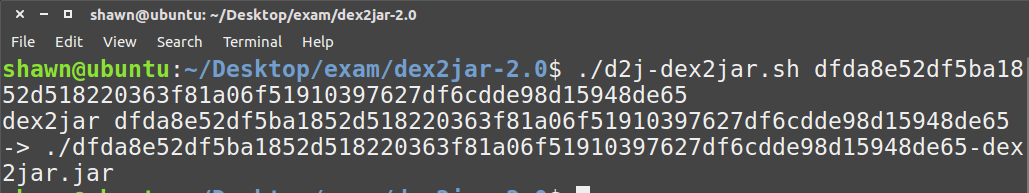
\includegraphics[scale=0.3]{dex2jar}
\caption{Using dex2jar on the xbot ransomware}
\label{fig:ra}
\end{figure}

The output is a jar file which can be opened in JD-GUI.
Using JD-GUI, the java files can be saved.

\begin{figure}[H]
\centering
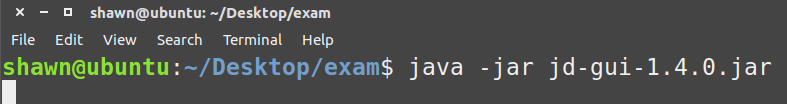
\includegraphics[scale=0.5]{jd-gui1}
\caption{Opening jar files using jd-gui}
\label{fig:ra}
\end{figure}

\begin{figure}[H]
\centering
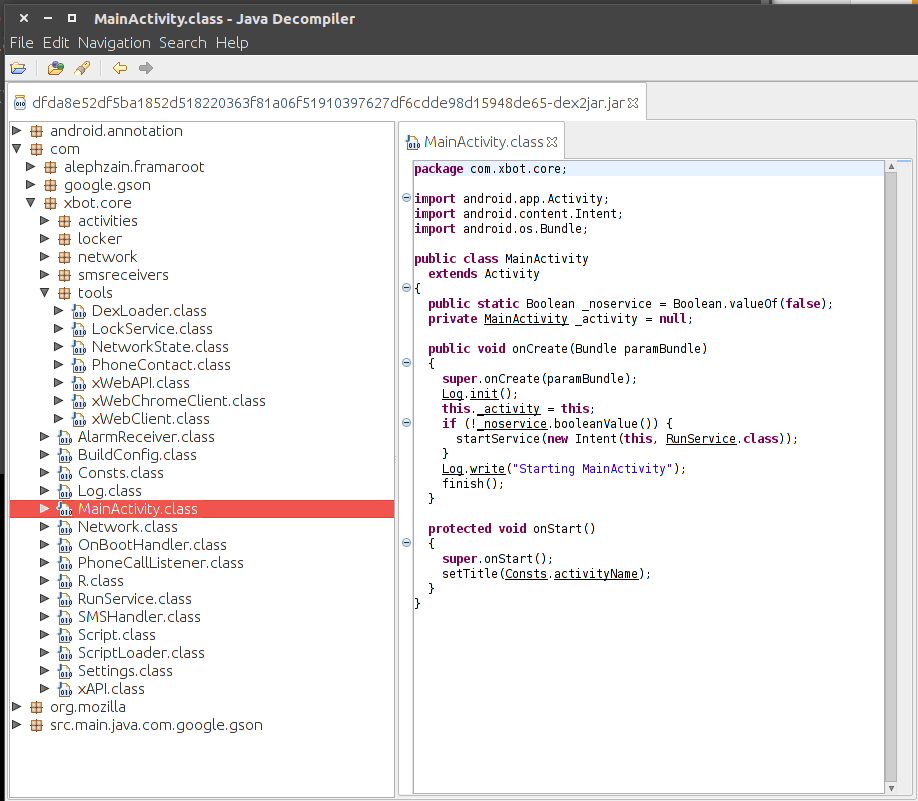
\includegraphics[scale=0.3]{jd-gui2}
\caption{jd-gui with all java files of xbot}
\label{fig:ra}
\end{figure}


After being installed on an Android device, Xbot contacts to the C2 server for further action.
Three of the actions was phising and one was activity hijacking.

\begin{figure}[H]
\centering
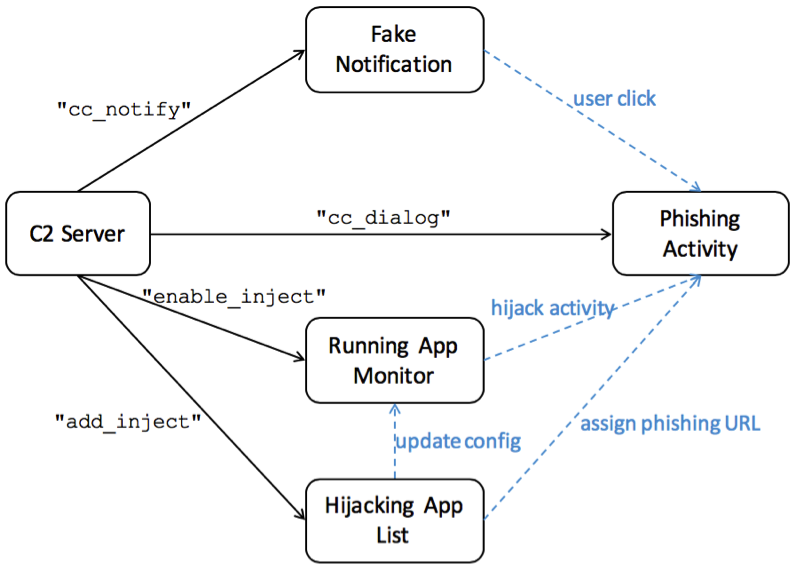
\includegraphics[scale=0.5]{xbot2}
\caption{Xbot's phising commands}
\label{fig:xbot2}
\end{figure}

When the C2 server gives a command of "cc\_notify", the app will display a notification based on ur location.
Which means if you are in Russia , then the notification will be in Russian language.
Rest of the world, it will be displayed in English.


\begin{figure}[H]
\centering
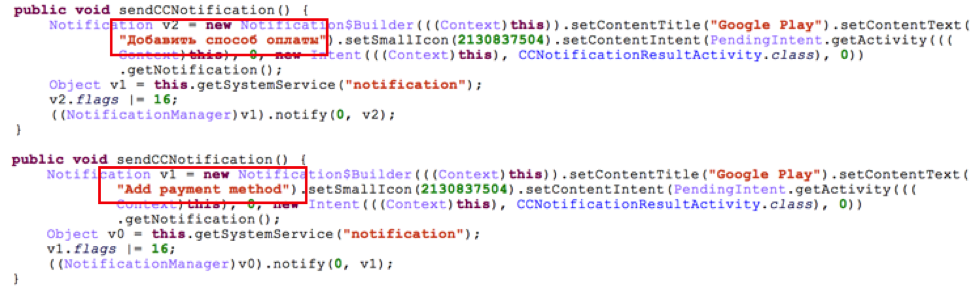
\includegraphics[scale=0.8]{xbot3}
\caption{Code for displaying the fake notification}
\label{fig:ra}
\end{figure}

Notification says that "add payment method" including the Google Play logo.
After clicking on the notification the user will be seeing a webpage in webview downloaded from the C2 server.
All the functionality is similar to the Google Play add payment method version.
All the information that the user gives will be saved to the C2 server.
The information saved are :-
\begin{itemize}
    \item credit card number
    \item expiration date
    \item CVV number
    \item card holder's name
    \item card holder's billing address
    \item card holder's phone number
    \item VBV (Verified by Visa) or McSec (MasterCard SecureCode) number
\end{itemize}

\begin{figure}[H]
\centering
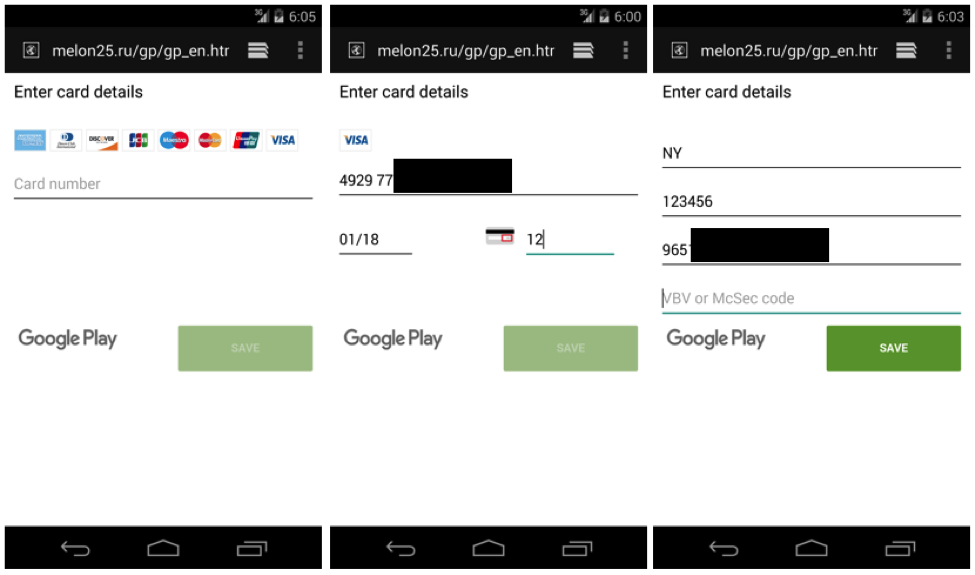
\includegraphics[scale=0.5]{xbot4}
\caption{Fake Google Play payment page}
\label{fig:ra}
\end{figure}

If the C2 command is "cc\_dialog", no notification will be displayed, the fake Google play add payment method page will be displayed.
If the C2 command is "enable\_inject", the app will check for all running apps using getRunningTasks() API in Android. 
They will search if there is any Google Play store app or one of the seven Australian app banks and immediately popup another activity on the top of the running app. 
This is called "activity hijacking".


\begin{figure}[H]
\centering
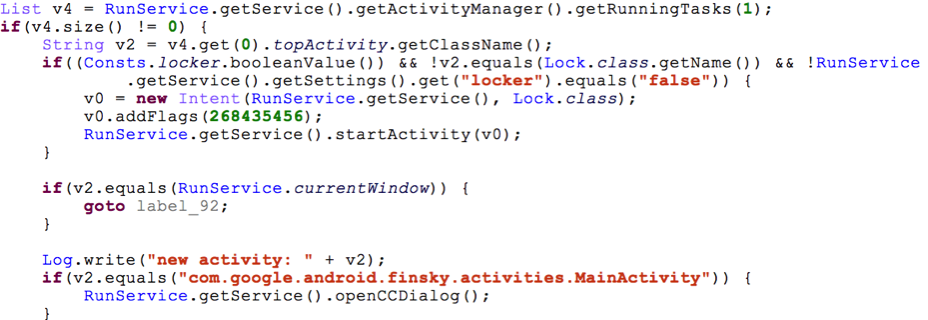
\includegraphics[scale=0.8]{xbot6}
\caption{Code for hijacking Google Play and banking apps}
\label{fig:ra}
\end{figure}

After installing xbot, it may ask for device administrator permissions.
If the C2 server sends "killon", the device will be set to silent mode and reset the password to "1811blabla".


\begin{figure}[H]
\centering
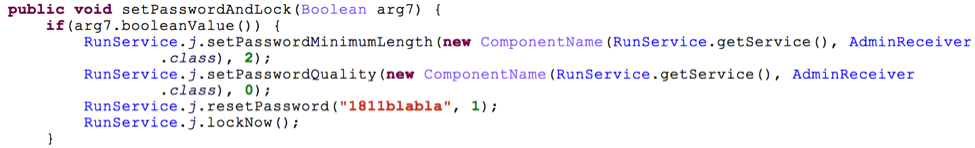
\includegraphics[scale=0.8]{xbot9}
\caption{Code to change the device password}
\label{fig:ra}
\end{figure}

If the C2 command is "enable\_locker", it will display the user that the phone is locked and files are encrypted.
The displayed thing is a webpage in webview from the address specified by the server.

\begin{figure}[H]
\centering
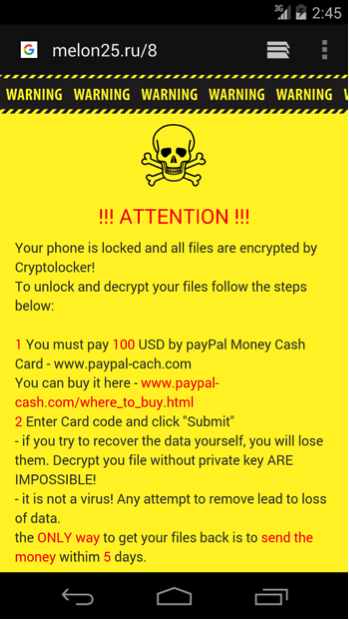
\includegraphics[scale=0.5]{xbot10}
\caption{Xbot ransom page}
\label{fig:ra}
\end{figure}

Xbot overrides onBackPressed(), onDestroy() and onPause() callback methods which makes the user to not get away from the page.
At the same time the xbot starts to encrypt the files in the external storage.
The encryption algorithm they used is XOR each byte of all files with an integer whose value is 50.

\begin{figure}[H]
\centering
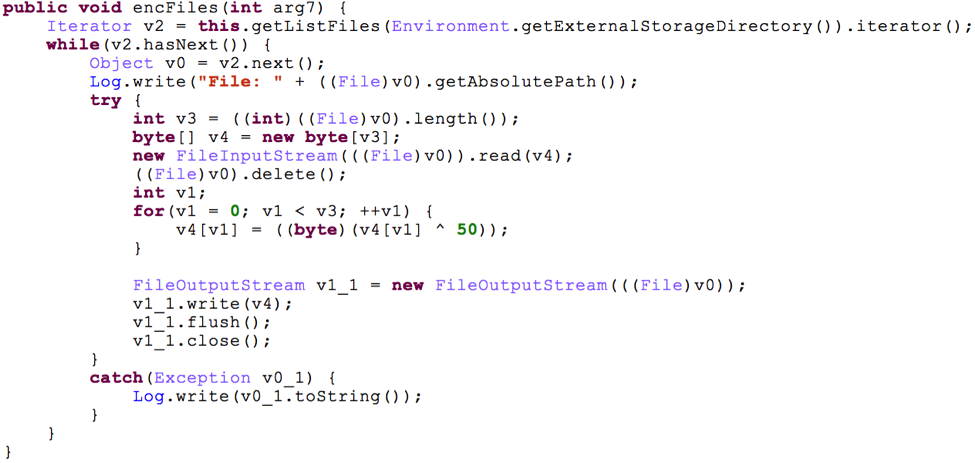
\includegraphics[scale=0.8]{xbot11}
\caption{Code to encrypt files in internal storage}
\label{fig:ra}
\end{figure}




\section{Detecting ransomwares using crowd sourcing App}

This section describes the working of Ransomware-CrowdSource app.
Source code of the app can be accessed at \href{https://github.com/jithin005/Ransomware-CrowdSource}{Ransomware-CrowdSource App}.
The main components of the Ransomware-CrowdSource app is 
\begin{itemize}
    \item Checker - is a broadcast reciever.
    \item Monitoring - is a service.
    \item Service - MyFirebaseMessagingService - is a service
    \item MainActivity - is an activity which acts as an interface to the user.
\end{itemize}

\subsection{Checker}

\par A broadcast receiver is a program that works on some broadcast message.
The broadcast message that checker will be looking for is \\
"android.intent.action.PACKAGE\_ADDED"
It keeps looking for any new app is installed.
If installed the app will be sent to the server along with the package name.



\subsection{Monitoring}

\par This is a service which keeps on getting the ip address that each app uses.
A service is similar to daemon in linux.
The ip address that it gets will saved to a flat file.
This flat files will be uploaded periodically, after successful sending the file will be deleted from the device.

\subsection{MyFirebaseMessagingService}

\par I used Firebase to communicate from the server to the device.
The Firebase creates an ID for each user, this will be saved in the database of the server.
This ID will be used to contact the registered devices.
If any malicious traffic or app is found it will send the message to delete the app with the app name.
Below is the image of the notification received by the user from the server if a malicious app is found. 

\begin{figure}[H]
\centering
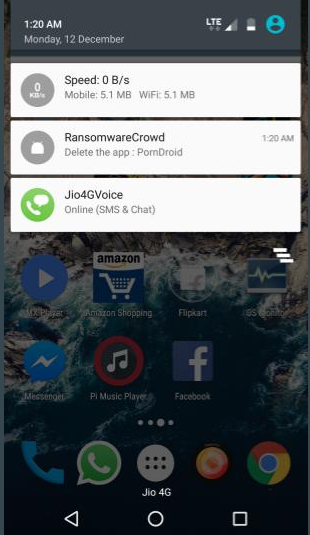
\includegraphics[scale=0.8]{notify}
\caption{Notification received by the registered device}
\label{fig:ra}
\end{figure}

\clearpage

\subsection{MainActivity}

\par This act as the user interface to the user.
This gives all the ip connections made by each app.
A screenshot of the MainActivity is shown below :-

\begin{figure}[H]
\centering
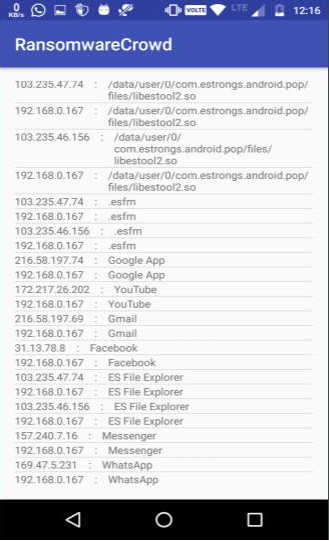
\includegraphics[scale=0.8]{front}
\caption{MainActivity with all app and its ip connections}
\label{fig:ra}
\end{figure}






\chapter{Related Work}


\par In \cite{andronio2015} ransomware was analysed statically. 
Where they used NLP (Natural Language Processing). 
It checked for all the strings and text to detect the threatening factor by comparing with sentence and words in many language. 
Thus there was a learning step where the framework learnt all the threatening words and sentences from most of the language. 
After this they used API flow to detect any file operation done similar by the ransomware. 
Ransomware, they takes each file and encrypts it and delete the original file. 
So they will check for the same flow to detect ransomware. 
Also they can detect Locker ransomware. 
Checks if the app is able to lock the phone by static analysis. 
Also it checks if home and back button are override to a user defined function. 
This framework does not work for languages which are not known to them, so it cant be used world wide. 
This framework doesn't check dynamically loaded APK files. 
If the ransomware app displays figures rather than text, this frame work fails as it does not use any OCR (Optical Character Recognition) techniques.


\par In \cite{yang2015} the author gives a basic idea about how to do automatic detection and analysis of ransomwares. 
This is a theoretical paper. 
This paper discusses about common hacking techniques like insecure WiFi, cloned apps, third party apps etc. 
Author also specifies that the permission also can give a hint if it is a ransomware or not. 
Specifies some combination of permission which is seen for ransomware. 
Design of an automated analysis which has both static and dynamic analysis. 
Static analysis includes checking of permissions, sequence of API invoking, checking the resources and APK structure.
Dynamic analysis includes critical path and data flow, malicious domain access, malicious charges and checks if it bypasses the android permission. 
This paper doesn't include any implementation just gives an idea about how to do the analysis.


\par In \cite{mercaldo2016} the author uses formal methods to detect ransomware. 
The paper boast on getting 100\% success in detecting ransomware but not much of implementation is given. 
The formal method, author used has three steps :-
\begin{itemize}
    \item \textbf{Formal method construction :-} Byte-code of the app is converted to a formal method.
    \item \textbf{Temporal Logic Properties Construction :-} Defines the behaviour of ransomware. Differentiates from goodware. 
    \item \textbf{Ransomware Family Detection :-} A formal verification environment, which contain a model checker. Logical properties are compared of the app and the ransomwares used for the logic properties construction.
\end{itemize}
Advantage of this implementation is that it is independent of languages. 
Source code is not needed for this proposed scheme.
Even if the source code is obfuscated, the proposed scheme will work.
Implementing such a scheme is very difficult as they have to define model for each category and to implement it in a device requires good amount of resource.


\par In \cite{scaife2016} the author focuses only on crypto ransomwares in PC running Windows, as most of the ransomware attack is reported in windows platform. 
Analysis was done on a data centric behavior.
Crypto ransomwares are categorised into three:-
\begin{itemize}
    \item \textbf{Class A:-} In this class of ransomware, there is no deletion of the original file.
    The encrypted data overwrites the existing data.
    \item \textbf{Class B:-} In this class of ransomware, the file to be encrypted is moved to a temporary place.
    Then it is overwritten with encrypted data. 
    Then it is moved back to the original position of the file.
    \item \textbf{Class C:-} In this class of ransomware, the original file is deleted.
\end{itemize}
When the file is encrypted, the file's extension changes.
This can be detected by keeping track of the magic number of the files.
The author introduces another technique, where it uses sdhash to compare two instance of same file.
The sdhash returns 100\% if the two files are same and if two files are fully different then it returns 0\%.
If the file's content is changed by a user then the sdhash of those two files will be greater than 50\% which shows some similarity.
If the crypto-ransomware encrypts the file, the file's content becomes completely random where sdhash  value is less than 50\%.
File-type funnelling is another indicator which author used for detecting ransomwares. 
Crypto ransomwares after encrypting changes the file extension to a single one. 
So a monitoring system can detect which process is using different type of files creating only a single type of files.


\par In \cite{song2016}, the author took a modular approach for preventing the ransomware from encrypting the files or locking the device.
Configuration, Monitoring and Processing modules are used.
In configuration module, the user is asked about which files are to be protected. 
This protected area is called Priority Protection Area(PPA).
Blacklisted process and system configuration is also noted
In monitoring module, the files and process are monitored for detecting anomalies.
Every file event is noted, for those files that is noted in PPA.
All the process that access the files in PPA is monitored also checking the memory usage, I/O count etc.
In processing module, whenever any malicious activity is detected from the monitoring module, this module will notify the user about it.
Whatever action taken by the user is noted by the app and added to the database.


\par In \cite{agarwal2013}, the author uses crowd sourcing for getting the privacy settings and protecting the privacy of the user.
The author introduced an app in iOS for protecting the privacy, name of the app is ProtectMyPrivacy(PMP).
This works by hooking into those function where privacy matters.
After hooking it implements the modules in the framework.
So whenever a private data is to be used, PMPSBTweak will be called.
This will check the PMP server for the settings if not available in the local database.
Whatever decision is to be made is sent to PMPSB Tweak.
If it is to be protected then the data is sent to an anonymizer module.
The PMP server contains all the privacy setting that is collected from the users of the app.

\chapter{Conclusion and Future Work}

In this report, we showed you how some elements can be crowd sourced from the device, running on Android, of registered user for detecting ransomware.
We showed the architecture for detecting ransomware.
Only the app level implementation was done, this can be integrated with the Android OS.
We implemented the crowdsourcing of ip address that each app connects and these are analysed to term it as ransomware.
As only analysing ip is not enough to term an app as a ransomware.



% Recommendations are optional.
% You may include recommendations as a major division if your
% subject matter and research dictate.
% Reference: TM 32.
% CHANGE NEXT LINE?
%\include{recommendations}

% Appendices are optional.
% Appendices are not necessarily part of every thesis. Appendices are used
% for supplementary illustrative material, original data, computer programs,
% and other material not necessarily appropriate for inclusion within the
% text of your thesis. 
% Reference: TM 33.
% Use "\appendix" for one appendix or "\appendices" for more than one
% appendix.
% CHANGE NEXT 7 LINES?
%\appendices
%\include{demo-citations}
%\include{demo-figures}
%\include{demo-mathematics}
%\include{demo-multicols}
%\include{demo-tables}
%\include{demo-text}

% Bibliography is required if you consulted any outside references.
% Reference: TM 32.
\bibliographystyle{unsrt}
%\bibliography{all}
\bibliography{ransomware}

\end{document}          
